    \subsection*{7.X.4 \quad The Gradient: a vector input, scalar output}
    
        Our plan is to look at every derivative combination of scalars, vectors, and matrices we can.
        
        First, we consider:
        
        \begin{equation}
            \pderiv{ \text{(Scalar) } } { \text{(Vector)} }
            =
            \pderiv{\red{s}}{ \pur{v} } 
        \end{equation}
        
        We'll take $\red{s}$ to be our scalar, and $\pur{v}$ to be our vector. So, our input is a \textbf{vector}, and our output is a \textbf{scalar}.
        
        \begin{equation}
            \Delta \pur{v}
            \longrightarrow
            \boxed{f}
            \longrightarrow
            \Delta \red{s}
        \end{equation}
        
        How do we make sense of this? Well, let's write $\Delta \pur{v}_i$ explicitly:
        
        \begin{equation}
            \overbrace{
                \begin{bmatrix}
                    \Delta \pur{v_1}\\ \Delta \pur{v_2}\\ \vdots \\ \Delta \pur{v_m}
                \end{bmatrix}
            }^{\Delta v}
            \longrightarrow 
            \Delta \red{s}
        \end{equation}
        
        We can see that we have $m$ different \textbf{inputs} we can change in order to change our \textbf{one} output.
        
        So, our derivative needs to have $m$ different \textbf{elements}: one for each element $\pur{v}_i$.
    
    \secdiv
       
    \subsection*{7.X.5 \quad Finding the scalar/vector derivative}
        
        But how do we shape our matrix? Let's look at our \textbf{rule}.
        
        \begin{equation}
            \Delta \red{s}
            \approx
            \pderiv{\red{s}}{ \pur{v} }  
            \star
            \Delta \pur{v}
                \qquad
                \text{or}
                \qquad
            \Delta \red{s}
            \approx
            \pderiv{\red{s}}{ \pur{v} } 
            \star
            \overbrace{
                \begin{bmatrix}
                    \Delta \pur{v_1}\\ \Delta \pur{v_2}\\ \vdots \\ \Delta \pur{v_m}
                \end{bmatrix}
            }^{\Delta v}
        \end{equation}
        
        How do we get $\Delta red{s}$? We have so many variables. Let's focus on them one at a time: breaking $\Delta \pur{v}$ into $\Delta \pur{v_i}$, so we'll try to consider each $\pur{v_i}$ \textbf{separately}.
            \note{It's usually possible to change each $\pur{v_i}$, so we have to look at every one of them.}
        
        One problem, though: how can we treat each \textbf{derivative} separately? Each $\Delta \pur{v_i}$ will move our position, which can change a different derivative $\pur{v_k}$: they can \textbf{affect} each other.
    
    \secdiv
    
    \subsection*{7.X.6 \quad Review: Planar Approximation}
        
        We'll resolve this the same way we did in chapter 3, \textbf{gradient} descent: by taking advantage of the "planar approximation".
        
        The solution is this: assume your function is \textbf{smooth}. The \textbf{smaller} a step you take, the \textbf{less} your derivative has a chance to change.
            \note{This isn't true for big steps, but eventually, if your step is small enough, then the derivative will barely change.}
        
        \miniex Take $f(x)=x^2$. 
        
        \begin{itemize}
            \item If we go from $x=1\rightarrow2$, then our derivative goes from $f'(x)=2 \rightarrow 4$.
            
            \item Let's \textbf{shrink} our step. We go from $x=1\rightarrow1.01$, our derivative goes from $f'(x)=2 \rightarrow 2.02$.
                \begin{itemize}
                    \item Our derivative is almost the same!
                \end{itemize}
        \end{itemize}
        
        if we take a small enough step $\Delta v_i$, then, if our function is \textbf{smooth}, then the derivative will hardly change!
            \note{You could imagine repeatedly shrinking the size of our step, until the change in the derivatives is basically unnoticeable.}
            
        So, if we zoom in enough (shrink the scale of change), then we can \textbf{pretend} the derivative is \textbf{constant}.\\
        
        \begin{concept}
            If you have a \gren{smooth function}, then...
            
            If you take sufficiently \vocab{small steps}, then you can treat the derivatives as \purp{constant}.
        \end{concept}
        
        \phantom{}\\
        
        \begin{clarification*}
            This section is \vocab{optional}.
            
            We can describe "sufficiently small steps" in a more mathematical way:
            
            Our goal is for $\org{f'(x)}$ to be \purp{basically constant}: it doesn't change much. $\Delta \org{f'(x)}$ is \gren{small}. 
            
            Let's say it can't change more then $\pur{\delta}$. 
            
            If you want 
            \begin{itemize}
                \item $\Delta \org{f'(x)}$ to be very small ($|\Delta \org{f'(x)}| < \pur{\delta}$)
                \item It has been proven that...
                \begin{itemize}
                    \item can take a small enough step $|\Delta \red{x}| < \pur{\epsilon}$, and to get that result.
                \end{itemize}
            \end{itemize}
        \end{clarification*}
        
        One way to describe this is to say that our function is (locally) \textbf{flat}: it looks like some kind of plane/hyperplane.
            \note{The word "locally" represents the small step size: we stay in the "local area".}\\
        
        \begin{clarification}
            Why is this \purp{true}? Because a \vocab{hyperplane} can be represented using our \vocab{linear} function 
            
            \begin{equation*}
                f(x) 
                \approx
                \red{\theta^T}x+\theta_0
                =
                \theta_0 + \red{\theta_1}x_1+\red{\theta_2}x_2+\dots+ \red{\theta_m}x_m
            \end{equation*}
            
            If we take a derivative:
            
            \begin{equation*}
                \pderiv{f}{x_i}
                =
                \theta_i
            \end{equation*}
            
            That derivative is a \purp{constant}! It's doesn't change based on \gren{position}.
        \end{clarification}
        
        \begin{figure}[H]
            \centering
                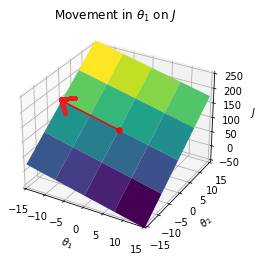
\includegraphics[width=70mm,scale=0.5]{images/gradient_descent_images/theta1_movement_plane.png}
            \caption*{If we take very small steps, we can approximate our function as \textbf{flat}.}
        \end{figure}
        
        
        Why does this help? If our derivative doesn't \textbf{change}, we can combine multiple steps  You can take multiple steps $\Delta \pur{v_i}$ and the order doesn't matter.
            \note{So, you can combine your steps or separate them easily.}
            
        \begin{figure}[H]
            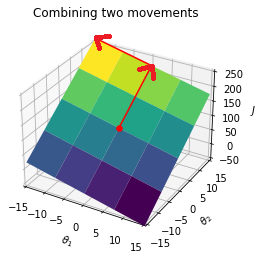
\includegraphics[width=70mm,scale=0.5]{images/gradient_descent_images/thetaboth_movement_plane.png}
            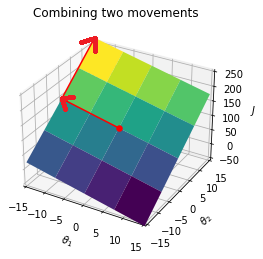
\includegraphics[width=70mm,scale=0.5]{images/gradient_descent_images/thetaboth_movement_plane_reversed.png}
                
            \caption*{We can break up our big step into two smaller steps that are truly independent: order doesn't matter.}
        \end{figure}
        
        
        
        With that, we can add up all of our changes:
        
        \begin{equation}
            \Delta s = 
            \Delta s_{\text{from } v_1}
            +
            \Delta s_{\text{from } v_2}
            +
            \dots
            +
            \Delta s_{\text{from } v_m}
        \end{equation}


    \subsection*{7.X.7 \quad Our scalar/vector derivative}
        
        From this, we can get an \textbf{approximated} version of the MV chain rule.\\
        
        \begin{definition}
            The \purp{multivariable chain rule} \vocab{approximation} looks similar to the multivariable chain rule, but for finite changes $\Delta x_i$.
            
            In 3-D, we get
            
            \begin{equation*}
                \Delta \red{f} 
                = 
                \overbrace{
                    \pderiv{\red{f}}{\pur{x}}
                    \Delta \pur{x}
                }^{\text{$x$ component}}
                +
                \overbrace{
                    \pderiv{\red{f}}{\pur{y}}
                    \Delta \pur{y}
                }^{\text{$y$ component}}
                +
                \overbrace{
                    \pderiv{\red{f}}{\pur{z}}
                    \Delta \pur{z}
                }^{\text{$z$ component}}
            \end{equation*}
            
            In general, we have
            
            \begin{equation*}
                \Delta \red{f} 
                \quad
                = 
                \quad
                \sum_{i=1}^{m}
                \overbrace{
                    \pderiv{\red{f}}   {\pur{x_i}}
                    \Delta \pur{x_i}
                }^{\text{$x_i$ component}}
            \end{equation*}
        \end{definition}
        
        This function lets us add up the effect each component has on our output, using \textbf{derivatives}.
        
        This gives us what we're looking for:
        
        \begin{equation}
            \Delta \red{s} 
            \quad
            \approx
            \quad
            \sum_{i=1}^{m}
            \pderiv{\red{s}}   {\pur{v_i}}
            \Delta \pur{v_i}
        \end{equation}
        
        If we circle back around to our original approximation:
        
        \begin{equation}
            \sum_{i=1}^{m}
            \pderiv{\red{s}}   {\pur{v_i}}
            \Delta \pur{v_i}
            \quad
            =
            \quad
            \pderiv{\red{s}}{ \pur{v} } 
            \star
            \overbrace{
                \begin{bmatrix}
                    \Delta \pur{v_1}\\ \Delta \pur{v_2}\\ \vdots \\ \Delta \pur{v_m}
                \end{bmatrix}
            }^{\Delta v}
        \end{equation}
        
        When we look at the left side, we're multiplying pairs of components, and then adding them. That sounds similar to a \textbf{dot product}.
        
        \begin{equation}
            \sum_{i=1}^{m}
            \pderiv{\red{s}}   {\pur{v_i}}
            \Delta \pur{v_i}
            \quad
            =
            \quad
            \overbrace{
                \begin{bmatrix}
                    \pderivslash{\red{s}}   {\pur{v_1}}\\ 
                    \\
                    \pderivslash{\red{s}}   {\pur{v_2}}\\ 
                    \\
                    \vdots \\ 
                    \\
                    \pderivslash{\red{s}}   {\pur{v_m}}
                \end{bmatrix}
            }^{\pderivslash{\red{s}}{ \pur{v} }}
            \cdot
            \overbrace{
                \begin{bmatrix}
                    \Delta \pur{v_1}\\\\ \Delta \pur{v_2}\\\\ \vdots \\\\ \Delta \pur{v_m}
                \end{bmatrix}
            }^{\Delta \pur{v} }
        \end{equation}
        
        This gives us our derivative: it contains all of the \textbf{element-wise} derivatives we need, and in a \textbf{useful} form!\\
        
        \begin{definition}
            If $\red{s}$ is a \redd{scalar} and $\pur{v}$ is an $(m \times 1)$ \purp{vector}, then we define the \vocab{derivative} or \vocab{gradient} $\pderivslash{\red{s}}{\pur{v}}$ as fulfilling:
            
            \begin{equation*}
                \Delta \red{s}
                =
                \pderiv{\red{s}}{\pur{v}}
                \cdot
                \Delta \pur{v}
            \end{equation*}
            
            Or, equivalently,
            
            \begin{equation*}
                \Delta \red{s}
                =
                \bigg(
                    \pderiv{\red{s}}{\pur{v}}
                \bigg)^T
                \Delta \pur{v}
            \end{equation*}
            
            \boxdiv
            
            Thus, our derivative must be an \blu{$(m \times 1)$} vector
            
            \begin{equation*}
                \pderiv{\red{s}}{\pur{v}}
                \;
                =
                \;
                \begin{bmatrix}
                    \pderivslash{\red{s}}   {\pur{v_1}}\\\\
                    \pderivslash{\red{s}}   {\pur{v_2}}\\\\
                    \vdots \\\\
                    \pderivslash{\red{s}}   {\pur{v_m}}
                \end{bmatrix}
                \;
                =
                \;
                \begin{bmatrix}
                    \bigpderiv{\red{s}}   {\pur{v_1}}\\ 
                    \\
                    \bigpderiv{\red{s}}   {\pur{v_2}}\\ 
                    \\
                    \vdots \\ 
                    \\
                    \bigpderiv{\red{s}}   {\pur{v_m}}
                \end{bmatrix}
            \end{equation*}
        \end{definition}
        
        We can see the shapes work out in our matrix multiplication:
        
        \begin{equation}
            \overbrace{
                \phantom{\bigg(}
                    \Delta \red{s}
                \phantom{\bigg)^T}
            }^{ (\org{1} \times \grn{1}) }
            =
            \overbrace{
                \bigg(
                    \pderiv{\red{s}}{\pur{v}}
                \bigg)^T
            }^{ (\org{1} \times \blu{m}) }
            \overbrace{
                \phantom{\bigg(}
                    \Delta \pur{v}
                \phantom{\bigg)^T}
            }^{ (\blu{m} \times \grn{1}) }
        \end{equation}
        